\documentclass[]{IEEEtran}

\title{Modellazione in VHDL di un modulo hardware basato sull'algoritmo XTEA}
\author{Vladislav Bragoi - VR436747}

\usepackage{graphicx}
\usepackage[utf8]{inputenc}
\usepackage[italian]{babel}
\usepackage{booktabs}
\usepackage{float}
\usepackage{caption}
\usepackage{minted}
\usepackage{url}
\usepackage{tikz}
\usetikzlibrary{shapes,arrows}
\newcommand{\signal}[1]{\textit{#1}}
\newcommand{\code}[1]{\texttt{#1}}
\renewcommand{\arraystretch}{1.2}
 % \setlength{\tabcolsep}{0.5em}SystemC
\begin{document}
\maketitle

\begin{abstract}
In questo documento vengono descritte le scelte progettuali adottate per implementare l'algoritmo eXtended TEA (XTEA) in
un modulo hardware, utilizzando il linguaggio di descrizione VHDL.

\end{abstract}

\section{Introduzione} \label{sec:intro}
Il progetto svolto ha l'obiettivo di sviluppare in VHDL sintetizzabile un modulo hw che implementi l'algoritmo XTEA per 
la cifratura/decifratura di due parole a 32 bit ciascuna, a partire da una versione gi\`a sviluppata precedentemente in 
SystemC a diversi livelli di astrazione.
Inoltre, tramite i principali tool di sintesi in commercio, eseguire la sintesi su una FPGA di riferimento quale la 
Xilinx PYNQ Z1 per verificare la corretta funzionalit\`a del modulo prodotto e toccare con mano i principali motivi per
i quali le tecniche di high level synthesis non vengono ancora oggi ampiamente impiegate.


\section{Background}
In questo progetto \`e stato utilizzato il linguaggio di descrizione hardware VHDL\cite{VHDL} per il design e la
progettazione del modulo hardware, mentre i concetti di High Level Synthesis (HLS) \cite{HLS} sono stati utilizzati
come confronto con una versione generata automaticamente a partire da una descrizione pi\`u algoritmica.
In particolare, i software utilizzati sono:
\begin{itemize}
	\item Mentor Graphics Modelsim, per il design e la simulazione del modulo hw,
	\item Xilinx Vivado per verificare che il modulo progettato sia sintetizzabile,
	\item Xilinx Vivado HLS per la generazione automatica dell'hardware digitale a partire da una descrizione ad alto 
			livello (ad esempio in C/C++) da confrontare con il risultato della sintesi logica.
\end{itemize}

\section{Metodologia applicata}
\subsection{Implementazione}
\begin{figure}[bt]
	\centering
	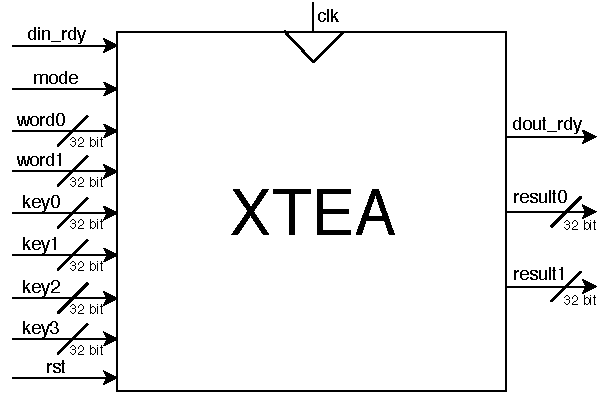
\includegraphics[width=0.6\columnwidth]{figures/xtea}
	\caption{Interfaccia del modulo}
	\label{fig:interf}
\end{figure}
L'implementazione in VHDL segue perfettamente la versione gi\`a implementata in SystemC, rispettando l'interfaccia del
modulo (in figura \ref{fig:interf}) e la scomposizione in FSM e DATAPATH gi\`a studiata precedentemente (visibile in 
figura \ref{fig:fsmd}).
\begin{figure}[bt]
	\centering
	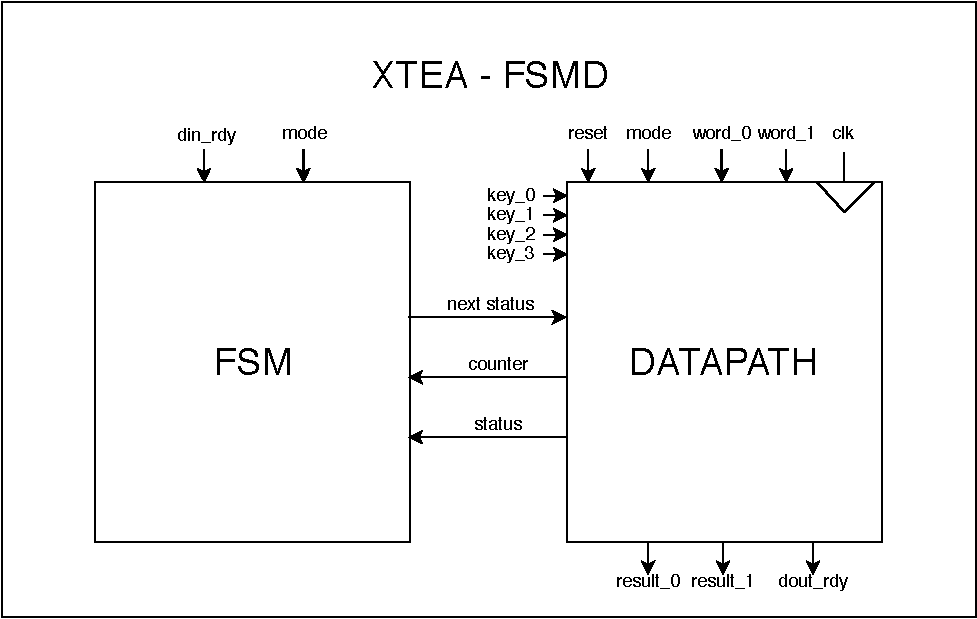
\includegraphics[width=0.9\columnwidth]{figures/fsmd}
	\caption{Scomposizione del modulo in fsm e datapath}
	\label{fig:fsmd}
\end{figure}
In particolare il componente presenta 6 ingressi a 32 bit ciascuno, di cui 4 per le chiavi da utilizzare durante la 
cifratura/decifratura e 2 per ricevere in ingresso le parole da cifrare/decifrare. Sono presenti inoltre i segnali di
\signal{din\_rdy}, \signal{mode} per selezionare la modalit\`a di esecuzione del modulo, \signal{rst} per il reset e 
\signal{clk} per il clock.
In output invece, il modulo restituisce il segnale di \signal{dout\_rdy} e 2 segnali a 32 bit per le parole 
cifrate/decifrate.
Di seguito l'interfaccia in VHDL:

\begin{minted}[fontsize=\footnotesize, tabsize=4]{VHDL}
entity xtea is
	port (
		clk         : in    bit;
		rst         : in    bit;
		mode        : in    bit;
		din_rdy     : in    bit;
		dout_rdy    : out   bit;
		key0        : in    unsigned (31 downto 0);
		key1        : in    unsigned (31 downto 0);
		key2        : in    unsigned (31 downto 0);
		key3        : in    unsigned (31 downto 0);
		word0       : in    unsigned (31 downto 0);
		word1       : in    unsigned (31 downto 0);
		result0     : out   unsigned (31 downto 0);
		result1     : out   unsigned (31 downto 0));
end xtea;
\end{minted}
Per quanto riguarda invece la fase di progettazione, i due processi \emph{fsm} e \emph{datapath} sono implementati per
rispettare lo schema rappresentato nella EFSM in figura \ref{fig:efsm}. In particolare il primo processo \`e sensibile 
ai segnali \signal{STATUS} e \signal{din\_rdy} e si occupa di aggiornare lo stato prossimo del sistema, mentre il secondo
processo, implementato rispettando lo stile 4 dei processi in VHDL, si occupa di aggiornare lo stato corrente del 
sistema, eseguire le operazioni logico-aritmetiche definite dall'algoritmo e infine scrivere il risultato sulle porte 
di output.

\subsection{Simulazione}
Per riuscire a simulare il modello, \`e necessario utilizzare il software Mentor Graphics Modelsim citato precedentemente.
I comandi da utilizzare, una volta creato un nuovo progetto e importati i due file \code{xtea.vhd} e \code{stimuli.do},
per lanciare la simulazione sono:

\AtBeginEnvironment{minted}{%
  \renewcommand{\fcolorbox}[4][]{#4}}
\begin{minted}[fontsize=\footnotesize, tabsize=1]{tcl}
	# carica il modello in sessione
	$ vsim work.xtea		
	# lancia lo script di simulazione
	$ do stimuli.do		
\end{minted}
Da notare che nello script di simulazione, oltre ad una prima fase di configurazione dei segnali su cui fare il tracing
grafico, viene eseguita una fase di soft reset del modulo. Questo per assicurarsi che il sistema riparta dallo stato 
iniziale previsto. Successivamente vengono assegnati alle varie porte del componente hw i valori desiderati. Ad esempio, 
per la cifratura vengono eseguiti i seguenti comandi per cifrare le parole esadecimali \emph{\code{12345678}} e 
\emph{\code{9abcdeff}}:

\AtBeginEnvironment{minted}{%
  \renewcommand{\fcolorbox}[4][]{#4}}
\begin{minted}[fontsize=\footnotesize]{tcl}
force word0 16#12345678 0 ns
force word1 16#9abcdeff 0 ns
force key0 2#01101010000111010111100011001000 0 ns
force key1 2#10001100100001101101011001111111 0 ns
force key2 2#00101010011001011011111110111110 0 ns
force key3 2#10110100101111010110111001000110 0 ns
force din_rdy 1 0 ns
force rst 1 0 ns
...
run 600 ns
\end{minted}
e la simulazione viene fatta durare 600 nanosecondi. Dopo circa 550 nanosecondi infatti, sul grafico (vedi figura 
\ref{fig:grafico}) \`e possibile vedere che il segnale \signal{dout\_rdy} \`e impostato a 1 e nelle porte di output 
\signal{result\_0} e \signal{result\_1} si trovano le due parole cifrate.
La simulazione completa è tracciata nel file \code{vsim.wlf}.

\subsection{Sintesi}
Per verificare che il modulo progettato fosse sintetizzabile \`e stato necessario utilizzare il tool Xilinx Vivado.
Una volta caricato il file \code{xtea.vhd} e impostata la piattaforma PYNQ \emph{\code{xc7z020clg400-1}} \`e stato 
possibile lanciare la sintesi, di cui ne viene riportato il risultato in figura \ref{fig:syn}. Dalla figura \`e 
possibile notare come la scelta di mantenere l'interfaccia gi\`a definita per la versione in SystemC ci richieda un 
utilizzo di 261 porte di I/O, risultando dunque non implementabile direttamente sulla FPGA scelta. In realt\`a questo 
limite pu\`o essere superato abbastanza tranquillamente se si utilizzano i registri della board, su cui mappare le porte
del circuito e sfruttando il bus AXI\cite{AXI} per una comunicazione diretta, oppure costruendo una versione diversa del
modello, avente un terzo processo che si occupa di caricare i valori sfruttando pi\`u cicli di clock e solo al 
completamento dell'operazione sbloccare gli altri due processi aggiornando i segnali a cui questi due sono sensibili.

\begin{figure}[tb]
	\centering
	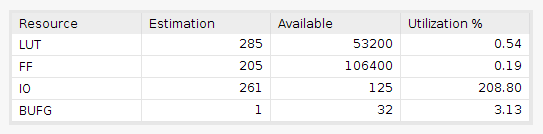
\includegraphics[width=0.9\columnwidth]{figures/syn_res.png}
	\caption{Utilizzo delle risorse su piattaforma PYNQ}
	\label{fig:syn}
\end{figure}

\subsection{Sintesi ad alto livello}
Per confrontare il codice sviluppato con uno generato automaticamente grazie alla sintesi ad alto livello, \`e stato
necessario utilizzare il tool Xilinx Vivado HLS gi\`a citato nelle sezioni sopra.
Questo tool ha permesso di generare automaticamente del codice VHDL a partire da un sorgente in C++ in cui l'algoritmo
veniva descritto ad alto livello. Il risultato della sintesi è visibile in figura \ref{fig:hls}.
Questa versione soffre comunque del problema relativo al sovrautilizzo delle porte di I/O, risultando non implementabile
direttamente sulla PYNQ. Si rivelano necessarie anche qui dunque le accortezze citate sopra.

\begin{figure}[tb]
	\centering
	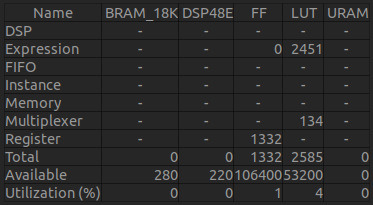
\includegraphics[width=0.7\columnwidth]{figures/syn_hls.png}
	\caption{Risultato della sintesi ad alto livello su piattaforma PYNQ}
	\label{fig:hls}
\end{figure}


\section{Risultati}
I risultati relativi all'implementazione del modulo hw in VHDL sono gi\`a stati in parte trattati precedentemente. La 
scelta di restare fedeli alla versione SystemC ha permesso un porting molto pi\`u rapido nel nuovo linguaggio ma ha 
richiesto qualche accortezza in pi\`u nella gestione dei vincoli legati alla piattaforma hardware di riferimento 
(ad esempio l'utilizzo delle risorse hardware disponibili). Con la simulazione inoltre, di cui rimando nuovamente alla 
figura \ref{fig:grafico} per un'analisi pi\`u dettagliata, \`e stato possibile verificare la correttezza 
dell'implementazione, passaggio fondamentale per un successivo deploy su una board effettiva quale la PYNQ Z1 utilizzata
nel tool di sintesi.

\section{Conclusioni}
Il confronto tra la versione del modulo XTEA sviluppato in VHDL e la versione derivante da una sintesi ad alto livello, 
ha permesso di capire come un codice automatico generalmente si presenta essere molto pi\`u complesso, impegnativo da 
gestire e mantenere, e soprattutto molto pi\`u oneroso dal punto di vista dell'utilizzo delle risorse hardware, dato che 
partendo da un codice ad alto livello, si hanno informazioni pi\`u generiche sul modello da costruire.
Questo \`e uno dei motivi che fanno s\`i che ancora oggi, nonostante i diversi tool in commercio, lo sviluppo diretto
venga preferito ad una versione automatizzata. Il modo migliore dunque per costruire un circuito digitale risulta essere 
quello percorso in questo documento, ovvero passare da una versione in C++/SystemC ad alto livello, ad una versione in 
VHDL/Verilog pi\`u dettagliata, verificando la correttezza del componente prodotto con simulazioni software e/o test 
diretti su hardware programmabile prima di un eventuale impiego su larga scala costruendo hardware specifico, almeno 
fino a quando le tecniche di high level synthesis non permettano di raggiungere la versatilit\`a di un codice costruito 
a mano.

\bibliographystyle{IEEEtran}
\bibliography{biblio}

\begin{figure*}[b]
	\centering
	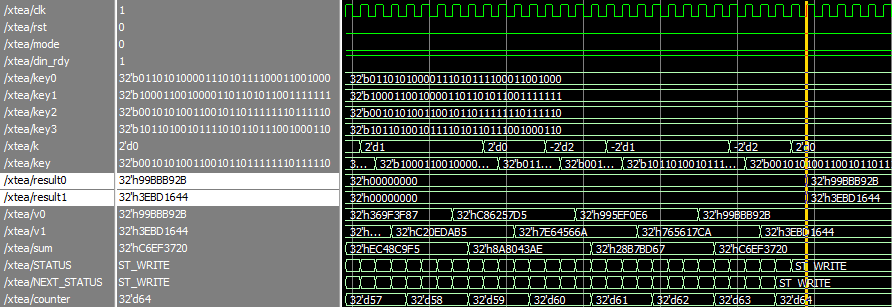
\includegraphics[width=0.8\textwidth]{figures/vhdl_exec}
	\caption{Esecuzione della cifratura delle parole \emph{\code{12345678}} e \emph{\code{9abcdeff}}}
	\label{fig:grafico}
\end{figure*}

\begin{figure*}[bt]
	\centering
	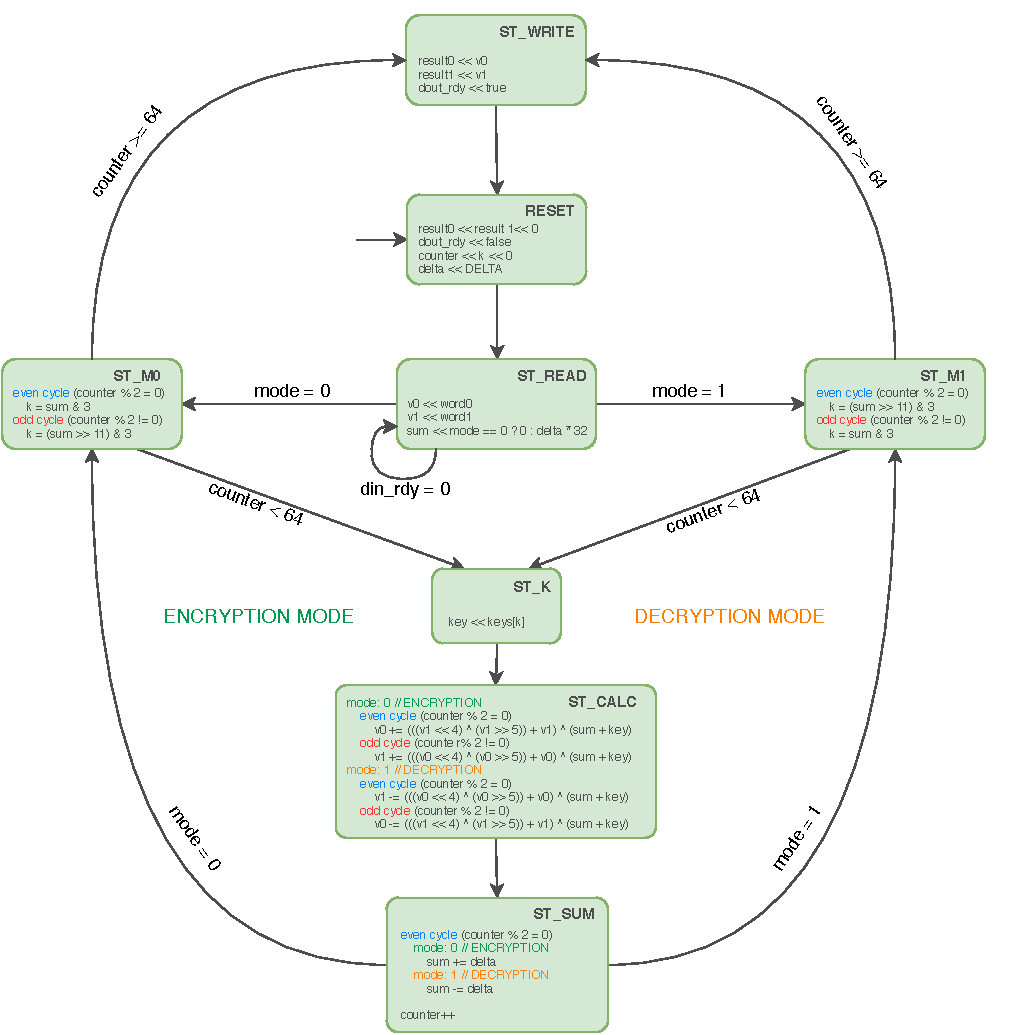
\includegraphics[width=0.7\textwidth]{figures/efsm.pdf}
	\caption{EFSM: rappresenta la completa funzionalit\`a del modulo}
	\label{fig:efsm}
\end{figure*}

\end{document}